%version of 11-22-18

\chapter{RECURRENCES}
\label{ch:Recurrences}

One of the intellectually most powerful strategies for all manner of
human endeavor is to ``learn from the past''---i.e., to {\em re}-use
knowledge that one has acquired earlier in order to acquire new
knowledge.  Within the domain of computing, this strategy is
exemplified by computations that derive the value of a function $F$ at
an argument $n \in \N^+$ by invoking the (hopefully, earlier-computed)
values of $F$ at arguments $1, 2, \ldots, n-1$.  The classical first
example of such a {\it recurrent} mode of computing involves the {\it
  factorial function} {\sc Fact} of Section~\ref{sec:unary-ops}.C.
\index{arithmetic!basic operations!factorial (of a nonnegative integer)}
The ``direct'' mode of computing {\sc Fact} at an argument $n \in
\N^+$ is:
\[ \mbox{\sc Fact}(n) \ = \ 1 \times 2 \times \cdots \times n. \]
The {\em recurrent} mode of computing {\sc Fact}($n$) is more
compact---and it better exposes the inherent structure of the
function.
\[ \mbox{\sc Fact}(n) \ = \ \left\{
\begin{array}{cl}
 n \times \mbox{\sc Fact}(n-1) & \mbox{ if } \ n > 1 \\
 1 & \mbox{ if } \ n = 1 \\
\end{array}
\right.
\]
This chapter is devoted to deriving and solving a variety of types of
recurrences.  In common with the rest of this text, our treatment of
this subject emphasizes exploiting recurrent structure in reasoning
and analysis: increased understanding will enable improved computing.


\section{Linear Recurrences}
\label{sec:linear-recurrences}
\index{linear recurrences}

This section is devoted to the solution of {\em linear} recurrences,
as exemplified by the following function specifications.  

\begin{equation}
\label{eq:Lin-Recur:general}
F(n) \ = \ \left\{
\begin{array}{cl}
a F(n/b) + f(n) & \mbox{for } n > b \\
1 & \mbox{for } n = b
\end{array}
\right.
\end{equation}

\begin{equation}
\label{eq:Lin-Recur:basic}
F(n) \ = \ \left\{
\begin{array}{cl}
a F(n/b) + c & \mbox{for } n \geq b \\
c & \mbox{for } n < b
\end{array}
\right.
\end{equation}

Myriad basic algorithmic problems, including sorting, selection,
matching, etc., can be solved using linear-recurrent algorithms
\cite{CLRS}---and such algorithms yield to specification and analysis
via linear recurrences.

In the next two subsections, we present analyses of recurrences
(\ref{eq:Lin-Recur:general}) and (\ref{eq:Lin-Recur:basic}).  The
reader will be able to extend the techniques we use in our analyses of
these specific recurrences in order to analyze other members of the
important family of linear-recurrent algorithms.


\subsection{The Simple Recurrence (\ref{eq:Lin-Recur:basic})} 
\label{sec:masterTheorem}
\label{sec:linear-recurrence-basic}

We focus first on the simpler of our sample recurrences, namely,
(\ref{eq:Lin-Recur:basic}).  Happily, there is a single perspicuous
proof that elegantly solves recurrences of this form.

By the time the reader has reached this paragraph, she has the
mathematical tools necessary to prove and apply what is called {\it
  The Master Theorem for Linear Recurrences} \cite{CLRS}.  The main
tools in the proof of the Theorem are: summing geometric summations
(Section~\ref{sec:geometric-sums}) and employing elementary asymptotic
notions and notations (Section~\ref{sec:asymptotics}).

\begin{theorem}[The Master Theorem for Linear Recurrences]
\label{thm:master-thm}
\index{The Master Theorem for Linear Recurrences}
Let the function $F$ be specified by the linear recurrence
(\ref{eq:Lin-Recur:basic}).  Then the value of $F$ on any argument $n$
is given by
\begin{equation}
\label{eq:Lin-Recur:solve}
\begin{array}{lcllll}
F(n) & = & (1 + \log_b n)c &  &  & \mbox{if } a=1 \\
     &   &                 &  &  & \\
     & = &
  {\displaystyle
  \frac{1-a^{\log_b n}}{1-a} \ \approx \ \frac{1}{1-a}
  }
                           &  &  & \mbox{if } a<1 \\
    &   &                  &  &  & \\
    & = &
  {\displaystyle
\frac{a^{\log_b n} -1}{a-1}
  }
                           &  &  & \mbox{if } a>1
\end{array}
\end{equation}
\end{theorem}

\begin{proof}
We expose the pattern generated by recurrence
(\ref{eq:Lin-Recur:basic}), by beginning to ``expand'' the specified
computation---replacing occurrences of $F(\bullet)$ as mandated in
(\ref{eq:Lin-Recur:basic}).  Once we discern the pattern, we jump to
the general form.
\begin{equation}
\label{eq:Lin-Recur:expand}
\begin{array}{lcccc}
F(n) & = & a F(n/b) + c & & \\
     & = & a \left( a F(n/b^2) + c \right) + c
             & = & a^2 F(n/b^2) + (a+1)c \\
     & = & a^2 \left( a F(n/b^3) + c \right) + (a+1)c
             & = & a^3 F(n/b^3) + (a^2+a+1)c \\
     &   & \vdots & & \vdots \\
     & = & 
{\displaystyle
\left(a^{\log_b n} + \cdots +a^2+a+1 \right) c
} & &
\end{array}
\end{equation}
The segment of (\ref{eq:Lin-Recur:expand}) ``hidden'' by the vertical
dots betokens an induction that is left to the reader.  Equations
(\ref{eq:geom-sum:b>1}) and (\ref{eq:geom-sum:b<1}) now enable us to
demonstrate that (\ref{eq:Lin-Recur:solve}) is the asserted
case-structured solution to (\ref{eq:Lin-Recur:basic}).  \qed
\end{proof}


\subsection{The More General Recurrence (\ref{eq:Lin-Recur:general})} 
\label{sec:linear-recurrence-general}

We now progress from the simple recurrence (\ref{eq:Lin-Recur:basic}) to
the more general recurrence (\ref{eq:Lin-Recur:general}).  We simplify
our problem in two ways, in order to avoid calculational complications
(such as floors and ceilings) that can mask the principles that govern
our analysis.
\begin{enumerate}
\item
We focus on the case $f(n) = n$.

It is a triviality to generalize to the slightly more ambitious $f(n)
= \alpha n + \beta$ (i.e., to a {\em linear} function $f$), but this
exension teaches no new lessons.
\item
We assume that the argument $n$ to functions $F$ and $f$ is a power of
$b$.

Removing this assumptions would significantly complicate our
calculations, but it would not change our reasoning.
\end{enumerate}

By ``unfolding'' (\ref{eq:Lin-Recur:general}) as in
Section~\ref{sec:linear-recurrence-basic}, we expose the algebraic
pattern created by the recurrence.  As in (\ref{eq:Lin-Recur:expand}),
once we discern this pattern, we jump to the general form (whch can be
verified via indution).
\[
\begin{array}{ccccc}
F(n) & = & a F(n/b) + n & & \\
     & = & a \left( a F(n/b^2) + n/b \right) + n
             & = & a^2 F(n/b^2) + (an/b+n) \\
     & = & a^2 \left( a F(n/b^3) + n/b^2 \right) + (a/b+1)n
             & = & a^3 F(n/b^3) + (a^2/b^2+a/b+1)n \\
     &   & \vdots & & \vdots \\
    & = & 
{\displaystyle
\left(a^{\log_b n} F(1) + \sum_{i=0}^{\log_b (n)-1} (a/b)^i \right) n
} & &
\end{array}
\]

We thus see that solving the more general recurrence
(\ref{eq:Lin-Recur:general}) requires only augmenting the solution to
the simpler recurrence (\ref{eq:Lin-Recur:basic}) by ``appending'' to
the simple solution a geometric summation whose base is the ratio
$a/b$.  The reader can now invoke the techniques from
Section~\ref{sec:summing-geometric-series:techniques} to arrive at a a
solution to (\ref{eq:Lin-Recur:general}).

When ``doing mathematics,'' one is often interested in discovering the
{\em dominant behavior} of the function $F(n)$ specified via a
recurrence such as (\ref{eq:Lin-Recur:general}).  An important lesson
to garner from the analysis we have been performing throughout this
section is the following:
\begin{itemize}
\item
When $a > b$, the behavior of $F(n)$ is dominated by the first
solution term
\[ a^{\log_b n} \cdot n \cdot  F(1) \ \ = \ \ n^{1 + \log_b a} \cdot F(1) \]
\item
When $a < b$, the behavior of $F(n)$ is dominated by the second
solution term
\begin{eqnarray*}
n \cdot \sum_{i=0}^{\log_b (n)-1} (a/b)^i
  & = &
\left( 1 \ - \  (a/b)^{\log_b (n)} \right) n \\
  & = &
n \ - \ a^{\log_b n} \\
  & = &
n \ - \ n^{\log_b a}
\end{eqnarray*}
\end{itemize}

One can learn yet more lessons about $F(n)$, specifically about how to
compute $F(n)$ (exactly or approximately) by observing the graphical
depiction in Fig.~\ref{fig:masterTheorem} of the calculation described
by recurrence (\ref{eq:Lin-Recur:general}).
\begin{figure}[htb]
\begin{center}
       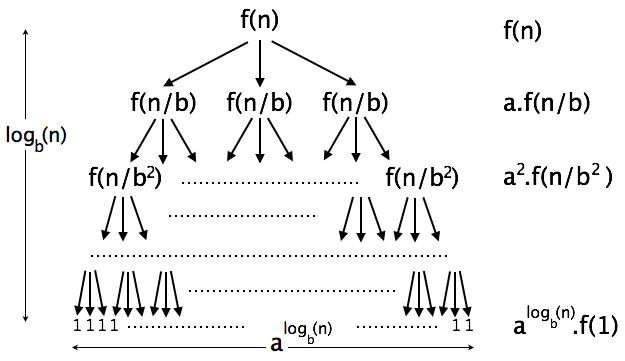
\includegraphics[scale=0.4]{FiguresMaths/MasterTheoremgeneral}
\caption{Development of the calculation specified by recurrence
  (\ref{eq:Lin-Recur:general}).  The associated summation appears on
  the right.
\label{fig:masterTheorem}}
\end{center}
\end{figure}
In particular, one observes in the figure that the computation---and
its associated tree---are perfectly balanced when $a=b$.  In
particular, when $a=b=2$, we obtain $F(n) = n \log_2(n)$.

{\Arny The notation in Fig.~\ref{fig:masterTheorem} (fonts, cdots)
  should be made consistent with the text.}


\section{Bilinear Recurrences}
\label{sec:bilinear-recurrences}
\index{bilinear recurrences}

\subsection{Binomial Coefficients and Pascal's Triangle}
\label{sec:binomial-coeff+Pascal}

In Section~\ref{sec:binomial-coeff}.C, we introduced and briefly
discussed the binomial coefficient \index{binomial coefficients}
$\displaystyle \Delta_{n,k} \ = \ {n \choose k}$ in its guise as a
binary operation on integers; see (\ref{eq:binom-coeff}).  And, we
established in Proposition~\ref{thm:manipulate-binom-coeff} the
summation rule
\[ {n \choose k} \ + \ {n \choose {k+1}} \ = \ {{n+1} \choose {k+1}} \]
for $\Delta_{n,k}$.  In fact, one can {\em define} binomial
coefficient via the {\em bilinear recurrence} that underlies this
rule.  This change in viewpoint is the topic of the current
subsection.

\subsubsection{Relating binomial coefficients with Pascal's Triangle}

Let us define the bivariate integer function\footnote{We alter our
  notation for binomial coefficients in deference to our change in
  viewpoint: We promote the integer pair $\langle n,k \rangle$ from a
  subscript to an argument, and we embellish $\Delta$ with a
  hat.}~$\hat{\Delta}(n,k)$ via the bilinear recurrence
\begin{equation}
\label{eq:binom-coeff-recurrence}
\hat{\Delta}(n,k) \ = \ 
\left\{
\begin{array}{cl}
1  & \mbox{ if } \ [n=1, k=0] \\
1  & \mbox{ if } \ [n=1, k=1] \\
\hat{\Delta}(n-1, k-1) \ + \  \hat{\Delta}(n-1,k) & \mbox{ otherwise}
\end{array}
\right.
\end{equation}

\smallskip

We claim that the function $\hat{\Delta}(n,k)$ thus defined is, in
fact, the for binomial coefficient $\displaystyle {n \choose k}$.  We
establish this claim with the help of a two-dimensional array of
integers known as {\it Pascal's Triangle},
\index{Pascal's triangle}
so named in honor of the French polymath Blaise Pascal.
\index{Pascal, Blaise}
Fig.~\ref{fig:pascal-triangle} provides a ``prefix'' of this famed
array, for $n,k \leq 5$.
\begin{figure}[htb]
\[
\begin{array}{c||r|r|r|r|r|r|r}
{\displaystyle {n \choose k}} & k=0 & k=1 & k=2 & k=3 & k=4 & k=5 &\ldots \\
\hline
\hline
n=1 & 1 & 1 &    &    &    &   & \ldots \\
\hline
n=2 & 1 & 2 & 1  &    &    &   & \ldots \\
\hline
n=3 & 1 & 3 & 3  & 1  &    &   & \ldots \\
\hline
n=4 & 1 & 4 & 6  & 4  & 1  &   & \ldots \\
\hline
n=5 & 1 & 5 & 10 & 10 & 5  & 1 & \ldots \\
\hline
\vdots &\vdots &\vdots &\vdots &\vdots &\vdots &\vdots &\ddots
\end{array}
\]
\caption{A ``prefix'' of Pascal's Triangle, for $n,k \leq 5$.}
\label{fig:pascal-triangle}
\end{figure}
The {\em formation rule of the array} is that the array-entry at (row
$n+1$, column $k+1$) is the sum of the array-entries at (row $n$, column
$k$) and at (row $n$, column $k+1$).
\index{Pascal's Triangle!formation rule}

\medskip

By comparing the formation rule for Pascal's Triangle with equation
(\ref{eq:add-binom-coeff}), you can anticipate the following result.

\begin{prop}
\label{thm:pascal-binom}
The entries of Pascal's Triangle are the binomial coefficients.
Specifically, for all $n,k$, the entry at (row $n$, column $k$) of the
Triangle is $\displaystyle {n \choose k}$.
\end{prop}

\begin{proof}
We note by observation and direct calculation (see
Fig.~\ref{fig:pascal-triangle}) that the proposition is true for $n =
1$ and $k \in \{0, 1\}$.  A simple double induction verifies that
every binomial coefficient appears in the Triangle and every Triangle
entry is a binomial coefficient.  \qed
\end{proof}

\noindent
****************** \\
induction on $n$, then for each value of $n$ on $k \leq n$ \\
{\Arny SHOULD WE SPELL THIS OUT IN DETAIL?  GIVE AS AN EXERCISE?} \\
******************

\subsubsection{Basic properties of the binomial coefficients}

We conclude this section with two results that expose important
aspects of the nature of binomial coefficients.  We begin with an {\it
  a priori} nonobvious observation that is rendered obvious by the
formation rule for Pascal's Triangle, in the light of
Proposition~\ref{thm:pascal-binom}.

\begin{prop}
\label{thm:binomcoeff-integer}
Every binomial coefficient is an integer.
\end{prop}
\index{binomial coefficients!integer-hood}

\begin{proof}
By the formation rule for Pascal's Triangle, every entry in that array
is obtained from integers via repeated additions.  This result
therefore follows from Proposition~\ref{thm:pascal-binom}'s proof that
the elements of the Triangle are precisely the binomial coefficients.  \qed
\end{proof}

\begin{prop}
\label{thm:sumsof-binomcoeff}
For every positive integer $n$,
\[
\sum_{i=0}^n \ {n \choose i} \ \ = \ \
{n \choose 0} \ + \ {n \choose 1} \ + \cdots + \ {n \choose {n-1}} \ +
\ {n \choose n} \ \ = \ \ 2^n
\]
\end{prop}
\index{binomial coefficients!summation formula}

\begin{proof}
The Binomial Theorem (Theorem~\ref{thm:Binomial-theorem}) tells us
that, for all $n \in \N$,
\[
(x+y)^n \ \ = \ \ \sum_{i=0}^n \ \ {n \choose i} x^{n-i} y^i.
\]
If we instantiate this polynomial equation with the values $x = y =
1$, then we obtain the present result.
\qed
\end{proof}


\subsection{The Fibonacci Sequence}
\label{sec:Fibonacci}
\index{Fibonacci sequence}
\index{Fibonacci numbers}

This section is devoted to one of the most storied topics in the world
of mathematics---in terms of the topic's manifestation in the real
world and in terms of the multiple names used to refer to its
discoverer,\footnote{Not surprisingly, this marvelous sequence was
  discovered many times, in many places.  Our story refers ony to its
  discovery in the West.}~the 13th-century Italian mathematician
variously known as: \index{Fibonacci, Leonardo}
\index{Fibonacci, Leonardo!alternative names}

\begin{tabular}{ll}
Fibonacci               & (Italian for: son of Bonaccio) \\
Leonardo of Pisa        & (his hometown) \\
Leonardo Pisano         & (variant of ``of Pisa'') \\
Leonardo Pisano Bigolo  & (his hometown plus family name) \\
Leonardo Fibonacci      & (for: son of Bonaccio Bigolo) \\
Leonardo Bonacci        & (for: son of Bonaccio Bigolo) \\
\end{tabular}

\medskip

\noindent
The sequence discovered by this multi-named genius is defined as follows.

\medskip

The {\it Fibonacci sequence}, or, {\it the Fibonacci numbers}, is an
infinite sequence
\[ F(0), \ F(1), \ F(2), \ \ldots \]
of elements of $\N^+$, the set of positive integers.  As just denoted,
we see that the numbers in the sequence are traditionally indexed by
elements of $\N$, the set of nonnegative integers and are often
written using functional ($F(i)$) notation rather than subscripts
($F_i$).  The classical definition of the sequence is as follows.
\index{Fibonacci sequence!definition}\index{Fibonacci numbers!definition}
\begin{eqnarray}
\nonumber
F(0) & = & 1 \\
\label{eq:Fibonacci-defn}
F(1) & = & 1 \\
\nonumber
F(n) & = & F(n-1) \ + \ F(n-2) \ \ \ \mbox{ for all } n > 1
\end{eqnarray}
The sequence is often specified just by listing its early elements:
\[ 1, \ 1, \ 2, \ 3, \ 5, \ 8, \ 13, \ 21, \ 34, \ \ldots \]


\subsubsection{The story of the Fibonacci numbers}
\label{sec:Fibonacci-story}
\index{Fibonacci sequence!story}
\index{Fibonacci numbers!story}

Leonardo Fibonnaci is said to have dscovered his eponymous sequence in
the course of contemplating the rate of population growth of
successive generations of an idealized immortal initial pair of
rabbits.  Rabbits mature quickly and, after attaining maturity at one
month, can spawn a new pair of progeny every following month.  So, at
``time $0$'', there is one pair of rabbits.  This persists at month
$1$, because there has not yet been time to produce new rabbits.  By
month $2$, though, there are $2$ pairs of rabbits.  At month $3$, only
the first pair will have spawned, so there are $3$ pairs of rabbits.
At month $4$, these $3$ pairs are joined by $2$ more.  The reader can
continue this story and discover that the number of pairs of rabbits
observed after successive months are given by the sequence generated
by the process implicit in recurrence (\ref{eq:Fibonacci-defn}) and
illustrated by our initial list.

The Fibonacci sequence's role in describing idealized rabbit
population statistics is no more fascinating than its appearance
elsewhere in the natural world---in structural features such as the
patterns of seeds in flower heads, the numbers of petals of flowers,
the growth patterns of pine cones and pineapples, and on and on; see
\cite{Basin63}.

The mathematical properties of this truly remarkable sequence will
occupy our attention in the remainder of this section.


\subsubsection{Fibonacci numbers and binomial coefficients}
\label{sec:FibNo+BinomCoeff}
\index{Fibonacci numbers!connection with binomial coefficients}
\index{binomial coefficients!connection with Fibonacci numbers}

%\begin{figure}[h]
%\begin{center}
%        \includegraphics[scale=0.4]{FIGmaths/DefFibo}
%        \caption{Principle of the Fibonacci progression}
%        \label{doublesum}
%\end{center}
%\end{figure}
%Notice that it is a special case of $u_{n+1} =\alpha.u_{n} + \beta.u_{n-1}$ for $\alpha=\beta=1$.
%\bigskip

There is a strong, nonobvious, connection between the binomial
coefficients of Section~\ref{sec:binomial-coeff+Pascal} and the
Fibonacci numbers of the current section.  We observe this connection
by contemplating the diagonals of Pascal's Triangle.  See
Fig.~\ref{fig:FiboPascal}.
\begin{figure}[htb]
\begin{center}
        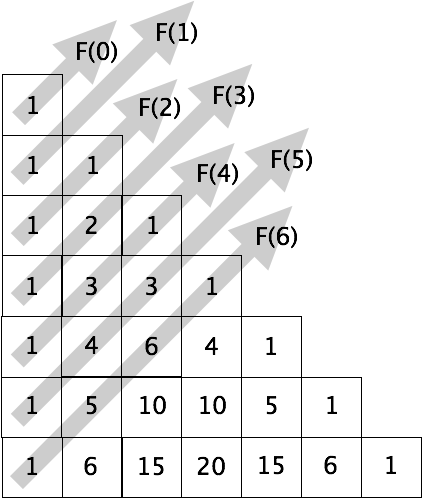
\includegraphics[scale=0.3]{FiguresMaths//FiboPascal1}
\caption{Obtaining Fibonacci numbers as diagonals of the left-justified Pascal Triangle.}
\label{fig:FiboPascal}
\end{center}
\end{figure}

\begin{prop}
\label{thm:FibNo+BinomCoeff}
For all $n \in \N$, the Fibonacci number $F(n)$ is the sum of the
first $\lceil (n+1)/2 \rceil$ binomial coefficients $\displaystyle {k
  \choose i}$ such that $k+i = n$.  Symbolically,
\begin{equation}
\label{eq:FibNo+BinomCoeff}
F(n) \ = \ {n \choose 0} \ + \ {{n-1} \choose 1} \ + \cdots + \ 
{{\lfloor (n+1)/2 \rfloor} \choose {\lceil (n+1)/2 \rceil -1}}.
\end{equation}
\end{prop}

\begin{figure}[htb]
\begin{center}
        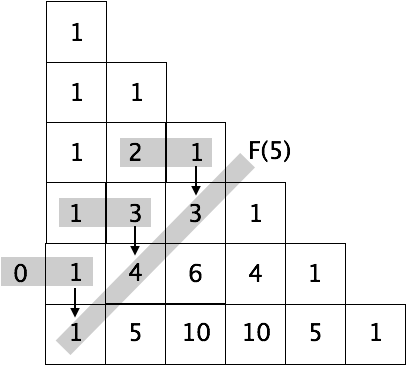
\includegraphics[scale=0.3]{FiguresMaths//FiboPascal2}
\caption{Each term of the diagonal is obtained by summing the two preceding ones.}
        \label{fig:FiboPascalExplanation}
\end{center}
\end{figure}

\begin{proof}[Sketch]
Because of the heavy calculational content of a complete proof, we
provide here just a short sketch.

Fig.~\ref{fig:FiboPascalExplanation} depicts a portion of Pascal's
Triangle with shaded diagonal and horizontal annotations.  The shaded
diagonal annotation depicts the three numbers in the Triangle that
sum to the Fibonnaci number $F(5)$.
\begin{enumerate}
\item
Looking at the three horizontal shaded areas {\em individually}
illustrates how each of the three numbers on the shaded diagonal,
being a binomial coefficient, arises as a sum of two numbers on the
preceding rowof the array---as instantiations of the formation rule
for Pascal's Triangle.  The illustrated instance of the rule asserts
that:
\[
\begin{array}{ccccccc}
{\displaystyle {5 \choose 0}}
 & = &
{\displaystyle 0 + {4 \choose 0} }
 & = &
0 + 1
 & = & 1 \\ \\
{\displaystyle {4 \choose 1}}
 & = &
{\displaystyle {3 \choose 0} + {3 \choose 1} }
 & = &
1 + 3
 & = & 4 \\ \\
{\displaystyle {3 \choose 2}}
 & = &
{\displaystyle {2 \choose 1} + {2 \choose 2} }
 & = &
2 + 1
 & = & 3
\end{array}
\]
\item
Looking at the three horizontal shaded areas {\em in tandem}
illustrates that the numbers along the shaded diagonal are sums of the
numbers along the two diagonals that are above the shaded one---as
instantiations of the formation rule for Fibonnaci numbers.  The
illustrated instance of the rule asserts that
\[ F(5) \ = \ F(4) + F(3) \ = \ 5 + 3 \ = \ 8. \]
\end{enumerate}

The preceding reasoning provides the infrastructure of an induction
that will prove that the proposition holds for every Fibonacci
number.  As suggested by the statement of the proposition, the
required calculations on indices can obscure the rather elegant basis
for the result.
\qed
\end{proof}

%Another way to write this relation is by the following expression:
%$F_n = binomial (n,0,1 ...)$


\subsubsection{Alternative generating recurrences for the Fibonacci sequence}
\label{sec:Fibonacci-other-recurrences}
\index{Fibonacci sequence!other generating recurrences}
\index{Fibonacci numbers!other generating recurrences}

Although the classical recurrence (\ref{eq:Fibonacci-defn}) is the
structurally simplest generator of the Fibonacci sequence, there exist
other generators that are not much more complex.  We now present two
other multi-linear recurrences that generate the sequence, in addition
to a family of binary generating recurrences.

\paragraph{\small\sf A. Two multi-linear generating recurrences}

\begin{prop}
\label{thm:FiboSum-1}
For all integers $n \geq 2$,
\begin{eqnarray}
\label{eq:multilinear-Fib-1}
F(n) & = &
1 \ + \ F(0) \ + \ F(1) \ + \ F(2) \ + \cdots + \ F(n-2) \\
\nonumber
     & = &
1 \ + \ \sum_{k=0}^{n-2} F(k)
\end{eqnarray}
\end{prop}

\begin{proof}
We proceed by induction.

\noindent
The {\em base case}, $n=2$, holds because $F(2) = 2 =  1 + F(0)$.

\noindent 
 Assume, {\em for induction}, that 
(\ref{eq:multilinear-Fib-1}) holds for all arguments $2 \leq n < m$.

\noindent
We {\em extend} the induction as follows.  Our inductive hypothesis
assures us that for all $m \geq 3$,
\[ F(m-1) \ = \ 1 \ + \ F(0) \ + \ F(1) \ + \ F(2) \ + \cdots + \ F(m-3). \]
Combining this with the classical recurrence
(\ref{eq:Fibonacci-defn}), we therefore have
\begin{eqnarray*}
F(m) & = & F(m-2) \ + \ F(m-1) \\
     & = &
F(m-2) \ + \ 1 \ + \ F(0) \ + \ F(1) \ + \ F(2) \ + \cdots + \ F(m-3)
\end{eqnarray*}

\noindent
This extends the induction and completes the proof.
\qed
\end{proof}

\medskip

While recurrence (\ref{eq:multilinear-Fib-1}) in
Proposition~\ref{eq:multilinear-Fib-1} employs all of the Fibonnaci
numbers up to the desired bound, recurrence
(\ref{eq:multilinear-Fib-2}) in the next proposition employs only
every other such number.

\begin{prop}
\label{thm:FiboSum-2}
For all integers $n \geq 2$,
\begin{eqnarray}
\label{eq:multilinear-Fib-2}
F(n) & = &
F(n-1) \ + \ F(n-3) \ + \ F(n-5) \ + \cdots + \ C(n) \\
\nonumber
\mbox{where} &   & \\
\nonumber
C(n) & = & \left\{
\begin{array}{cl}
F(2) + F(1) = 3  & \mbox{\rm if } \ n \ \mbox{\rm is even} \\
F(1) + F(0) = 2  & \mbox{\rm if } \ n \ \mbox{\rm is odd}
\end{array}
\right.
\end{eqnarray}
We thereby sum every other term up to the $(n-1)$th and use a
``clean-up'' term $C(n)$ to complete the sum.
\end{prop}

\begin{proof}
We develop the claimed summation (\ref{eq:multilinear-Fib-2}) by
iteratively expanding the righthand term ($F(n-2)$) of the classical
recurrence (\ref{eq:Fibonacci-defn}).  This expansion begins
\begin{eqnarray}
\label{eq:multilinear-Fib-3}
F(n)
& = &
F(n-1) \ + \ F(n-2) \\
\nonumber
& = &
F(n-1) \ + \ F(n-3) \ + \ F(n-4) \\
\nonumber
& = &
F(n-1) \ + \ F(n-3) \ + \ F(n-5) \ + \ F(n-6)
\end{eqnarray}
We continue this expansion process as long as we can, and then we add
a single {\em clean-up term}, which we have designated $C(n)$ in the
statement of the proposition.

Determining the value of $C(n)$ is facilitated by noticing that our
expansion is ``trying'' to have all term-indices in the expanded
summation have the same parity.  To wit, the successive indices of the
expanded summation differ by $2$, beginning with $n-1$, $n-3$, $n-5$,
and so on; therefore, the index $n-k$ that we expand always has the
same parity as $n$.  Let us observe the consequence of this fact for
the ``end game'' of the expanson process.
\begin{itemize}
\item
When $n$ is even, our expansion eventually comes down to
\[ \begin{array}{cl}
  & \cdots + F(5) \ + \ F(4) \\
\longrightarrow 
  & \cdots + F(5) \ + \ F(2) \ + \ F(1) \\
\end{array}
\]
The expansion must end at this point because we have run out of
Fibonacci numbers!  We therefore have
\[ C(n) \ = \ F(2) \ + \ F(1) \ = \ 2 + 1 \ = \ 3. \]

\item
When $n$ is odd, our expansion eventually comes down to
\[ \begin{array}{cl}
  & \cdots + F(4) \ + \ F(3) \\
\longrightarrow
  & \cdots + F(4) \ + \ F(1) \ + \ F(0)
\end{array}
\]
The expansion must end at this point because we have run out of
Fibonacci numbers!  We therefore have
\[ C(n) \ = \ F(1) \ + \ F(0) \ = \ 1 + 1 \ = \ 2. \]
\end{itemize}
In either case, our expanded summation produces the correct value of
$F(n)$.  \qed
\end{proof}


\paragraph{\small\sf B. A family of binary generating recurrences}

What we have earlier called ``generating recurrences'' or ``formation
rules'' for binomial coefficients and Fibonacci numbers can also be
viewed as (mathematical) identities on the quantities of interest.  In
our usage, the line between ``generating recurrences'' and
``identities'' centers on computational issues: multilinear
recurrences can feasibly be used to generate the desired numbers;
nonlinear recurrences such as we expose in this subsection will likely
not be used as generators.  Indeed, for several of the results we
cover here, it is the methodology of proof and analysis that we wish
to stress.

\begin{prop}
\label{thm:Fib-higher-indices}
For all $n \in \N$ and $k < n$
\begin{equation}
\label{eq:Fib-higher-indices}
F(n) \ = \ F(k) \cdot F(n-k) \ + \ F(k-1) \cdot F(n-k-1).
\end{equation}
\end{prop}

Of course, the classical recurrence (\ref{eq:Fibonacci-defn}) is
instance $(k = 1)$ of the family of recurrent equations
(\ref{eq:Fib-higher-indices}).

\begin{proof}
We first explain how one might guess at the existence of the family of
recurrences (\ref{eq:Fib-higher-indices}), and then we validate the
recurrences in the family.

We begin with the classical recurrence (\ref{eq:Fibonacci-defn})
and iteratively use this recurrence to ``expand'' the classical
recurrence.  In detail, we begin by combining the first two instances
of (\ref{eq:Fibonacci-defn}), namely,
\[
\begin{array}{lcrrr}
F(n)   & = & F(n-1) & + & F(n-2) \\
F(n-1) & = & F(n-2) & + & F(n-3)
\end{array}
\]
and we combine them algebraically to produce the following.
\[ F(n) \ = \ 2 F(n-2) \ + \ F(n-3). \]
And then we iterate!  The following table illustrates the result of
the first four iterations of the process.
\[
\begin{array}{ccrcrcrcrcrcr}
F(n) & = & F(n) & + & F(n-1) \\
     & = &      &   & 2 F(n-1) & + & F(n-2) \\
     & = &      &   &          &   & 3 F(n-2) & + & 2 F(n-3) \\
     & = &      &   &          &   &          &   & 5 F(n-3) & + & 3 F(n-4)  \\
     & = &      &   &          &   &          &   &          & + & 8
F(n-4) & + & 5 F(n-5)  \\
 & \vdots  &  & \vdots  &  &  \vdots &  & \vdots
 &  & \vdots  &   & \vdots  & 
\end{array}
\]
Note that the coefficients of the successive occurrences of the
Fibonacci numbers $F(i)$ that occur in our table are themselves
Fibonacci numbers.  By analyzing the emerging pattern---{\em remember
  our advice in Chapter~\ref{ch:doingmath} to always look for
  patterns}---we arrive at the family (\ref{eq:Fib-higher-indices})
of recurrent equations.

{\em Keep in mind that, at this point, we are still in the realm of
  conjecture!  We must now verify the universal validity of the
  family.}

We proceed by induction on the number $k$ of iterated expansions of
the classical recurrence (\ref{eq:Fibonacci-defn}).

The {\em basis for our induction} resides in the observation we shared
right after stating the proposition: Instance $(k = 1)$ of the posited
family of recurrent equations is just the classical recurrence
(\ref{eq:Fibonacci-defn}).

Let us assume that instance $k$ of family
(\ref{eq:Fib-higher-indices}), namely, the equation
\[ F(n) \ = \ F(k) \cdot F(n-k) \ + \ F(k-1) \cdot F(n-k-1) \]
is valid, and let us observe the result of producing instance $k+1$
from this instance.  We algebraically combine the just-cited equation
with the following instantiation of the classical recurrence:
\[ F(n-k) \ = \ F(n-k-1) \ + \ F(n-k-2) \]
We find that
\begin{eqnarray*}
F(n) & = & F(k) \cdot F(n-k) \ + \ F(k-1) \cdot F(n-k-1) \\
     & = & F(k) \cdot \big( F(n-k-1) \ + \ F(n-k-2) \big)  \ +
             \ F(k-1) \cdot F(n-k-1) \\
     & = & \big( F(k) \ + \ F(k-1) \big) \cdot F(n-k-1) \ + \ F(k)
             \cdot F(n-k-2) \\
     & = & F(k+1) \cdot F(n-k-1) \ + \ F(k) \cdot F(n-k-2)
\end{eqnarray*}
The induction is thus extended, which establishes the proposition.
\qed 
\end{proof}

\subsubsection{Toward a close form of the current term of the sequence}

In this section, we present the general methodology for determining
the close form of $F(n)$, that is an direct expression that only
depends on $n$ and not on the other terms of the sequence.  The
characteristic equation of $F(n+2) - F(n+1) - F(n) =0$ is:

$x^2 - x - 1 = 0$

Let determine its discriminant: $\Delta = 5$.
Since it is positive, this equation has two distinct roots:

$\Phi = \frac{1+\sqrt{5}}{2}$ and $\Phi' = \frac{1-\sqrt{5}}{2}$

The first one $\Phi$ is known as the \textit{golden ratio}. 

The general term $F(n)$ is equal to $a.\Phi^n + a'.\Phi'^n$ where $a$
and $a'$ are determined by two particular values $n=0$ and $n=1$:

$F(n)= \frac{1}{\sqrt{5}} ((\frac{1+\sqrt{5}}{2})^n - (\frac{1-\sqrt{5}}{2})^n)$


\subsection{Enrichment: Relatives of the Fibonacci Numbers}

\subsubsection{Profile numbers}

Profile numbers \cite{Rosenberg79}

\[ P(n+1, k+1) \ = \ P(n,k) + 2 P(n, k-1) \ \ \ k>0 \]

\[ \sum_{k=0}^{2n-1} \ = \ 3^n -1 \]

\[ P(n,k) \ = \ 2^{k-n} \cdot \sum_{i=0}^{2n-k} {n \choose i} \]


\begin{eqnarray*}
P(n, k+1) & = & 
  2 P(n,k) - 2^{k-n+1} {n \choose {k-n+1}} \\
P(n+1, k) & = &
  P(n,k) + 2^{k-n-1} \left[ {n \choose {k-n}} + {{n+1} \choose {k-n}} \right]
\end{eqnarray*}


\subsubsection{Lucas numbers}

The Lucas' sequence...

A natural question is what happens if we change the first ranks of the sequence keeping the same recurrence pattern?
It has been studied by the french mathematician Edouard Lucas, starting at 2 and 1. 
For some reasons that will be clarified later, the sequence is shifted (we take the convention $L(-1)=2$).

{\Denis do you agree with this shift of the sequence? it simplifies several proofs...}
\bigskip

\noindent
{\bf Definition.}
Given the two numbers $L(0) = 1$ and $L(1) = 3$, 
all the other Lucas numbers are obtained by the same progression as Fibonacci: 
$L(n+1) = L(n)+L(n-1)$.
\bigskip

n: 0, 1, 2, 3, 4, 5, 6, 7, 8, 9, ...

F(n): 1, 1, 2, 3, 5, 8, 13, 21, 34, 55, ...

L(n): 1, 3, 4, 7, 11, 18, 29, 47, 76, 123, ...
\bigskip

There are several interesting links with Fibonacci numbers.

In particular, we established at the beginning of this chapter in
Proposition~\ref{thm:FiboSum-1} that $F(n+2) = 1+ \sum_{k=0}^{n}
F(k)$.

We have similarly: $L(n+2) = 1+ \sum_{k=-1}^{n} L(k)$ since the basic step of the induction is still valid: $L(2) = L(-1 )+L(0) +1 = 2+1+1 = 4$.
%Actually, it will be true for all the progressions where $u_1=1$.
\bigskip

We can also easily show that the Lucas number of order $n$ is the sum of two Fibonacci numbers:

\noindent \textbf{Property. } 
\label{prop:Lucas1}
$L(n) = F(n-1)+F(n+1)$ for $n \geq 1$
\medskip


The proof is by induction as follows.

\begin{itemize}
\item
The \textbf{basis case} (for $n=2$) is true since $L(1) = 3 = F(2) + F(0) = 2+1$.

\item
\textbf{Induction step:} Let assume the property holds at all ranks $k \leq n$ and compute $L(n+1)$:

Apply the definition of Lucas' numbers: $L(n+1) = L(n)+L(n-1)$

Apply the induction hypothesis on both terms:

 $L(n+1) = F(n+1)+F(n-1)+F(n)+F(n-2)$
 
Apply now the definition of Fibonacci numbers for $F(n+1) + F(n) = F(n+2)$  and $F(n-1) + F(n-2) = F(n)$
and replace them in the previous expression:

$L(n+1) = F(n+2)+F(n)$
which concludes the proof.

%
\end{itemize}
\medskip

Notice that using a similar proof, we obtain $L(n) = F(n+2)+F(n-2)$. 
However, the generalization it is no more true for the further terms.
The interested reader can easily prove:

$L(n) = \frac{1}{2} (F(n+3)+F(n-3))= \frac{1}{3} (F(n+4)+F(n-4))$, and so on.
\medskip

Another interesting expression is the following.

\noindent \textbf{Property. } 
\label{prop:Lucas2}
$F(n+1) = \frac{1}{2} (F(1).L(n) + F(n).L(1))$


\medskip
The proof comes from direct arithmetic manipulations:

$2.F(n+1) = F(n+1) +  F(n+1) =  F(n+1) + F(n) + F(n-1)$

$= L(n) + F(n) $

$= F(1).L(n) + F(n).L(1)$
\medskip


The previous property can be extended for any $m>1$ as follows:

\noindent \textbf{Property. } 
\label{prop:Lucas3}
$2.F(n+m) = F(m).L(n) + F(n).L(m)$

The proof is left to the reader.

\bigskip

\noindent \textbf{Corollary:} Another interesting expression is
$F(2n) = F(n).L(n)$

The proof is straightforward using the previous expression for $m=n$, we get $2F(2n) = F(n).L(n) + F(n).L(n) = 2.F(n)L(n)$.




 


\subsubsection{Computing the product of two consecutive Fibonacci numbers}

\noindent \textbf{Property.} 
\label{prop:FiboSumConsecutive}
$F(n).F(n-1)= \sum_{k=0}^{n-1} F(k)^2$ (for $n \geq 1$)

\begin{itemize}

\item The relation  
can be proved very easily by the geometric argument shown in Fig.~\ref{fig:fibosquare}). 

\begin{figure}[h]
\begin{center}
        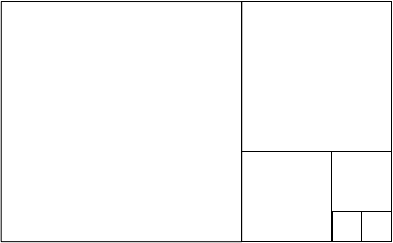
\includegraphics[scale=0.5]{FiguresMaths//Fiboembedded}
        \caption{Geometric interpretation of the relation $F(n).F(n-1)$.}
        \label{fig:fibosquare}
\end{center}
\end{figure}

\item
Another proof is by induction.

\begin{itemize}
\item
The \textbf{basis case} is to check $F(0).F(1) = F(0)^2$, which is true.

\item
\textbf{Induction step:} Let assume this property holds at rank $n$ and compute $F(n+1).F(n)$.

Apply the definition of $F(n+1)$:

 $F(n+1).F(n) =  (F(n)+F(n-1)).F(n) = F(n)^2 +  F(n).F(n-1)$
 
 Apply now the induction hypothesis to this last term:
 
 $F(n+1).F(n) = F(n)^2 + \sum_{k=0}^{n-1} F(k)^2 = \sum_{k=0}^{n} F(k)^2$.
 \end{itemize}

\end{itemize}

\subsubsection{Another property dealing with squares}

We will show the following property by two different methods

\noindent \textbf{Property.} 
\label{prop:FiboEmbedded}
$F(n+2)^2 = 4.F(n).F(n+1) + F(n-1)^2$ for $n \geq 2$.


The geometrical proof is obtained as depicted in Fig.~\ref{fig:fibosquareembedded} for computing $F_{n+2}^2$.

\begin{figure}[h]
\begin{center}
        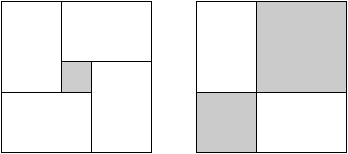
\includegraphics[scale=0.5]{FiguresMaths//FiboSquares}
        \caption{Geometric interpretation for computing $F_{n+2}^2$.}
        \label{fig:fibosquareembedded}
\end{center}
\end{figure}

Let remark that this figure might be adapted to show several properties using various decompositions of the squares and rectangles.

Another proof uses directly the definition of the Fibonacci numbers:

%$F_{n+1} + F_{n}$

$F(n+2)^2 = (F(n+1) + F(n))^2 $

$= F(n+1)^2+2.F(n+1).F(n)+F_{n}^2$

$= 4.F(n+1).F(n) - 2.F(n+1).F(n) + F(n+1)^2 + F(n)^2$

$= 4.F(n+1).F(n) + (F(n+1) - F(n))^2$

Again, using the definition of $F(n+1)$ into the square, we get the expected result:

$F(n+2)^2 = 4.F(n+1).F(n) + F(n-1)^2$


\subsubsection{Cassini's identity}

\noindent \textbf{Property. (Cassini's identity)} 
\label{prop:cassini}
$F(n-1).F(n+1) = F(n)^2 + (-1)^{n+1}$ for $n \geq 1$.


The proof by induction is as follows:

\begin{itemize}
\item 
The \textbf{basis case} is straightforward since $F(0).F(2) = 2$ and $F(1)^2 +1 = 2$.

\item
The \textbf{induction step} is proved assuming the Cassini's identity holds at rank $n$.

Apply the definition of $F(n+2)$:
 
$F(n).F(n+2) = F(n) (F(n+1)+F(n)) = F(n)^2 + F(n).F(n+1))$

Replace the last term using the recurrence hypothesis:

$F(n)^2 = F(n-1).F(n+1) - (-1)^{n+1} =F(n-1).F(n+1) + (-1)^{n+2} $

Thus,
$F(n).F(n+2) = F(n).F(n+1) + F(n-1).F(n+1) + (-1)^{n+2} = F(n+1) (F(n) + F(n-1)) + (-1)^{n+2}$ 

Apply again the definition of Fibonacci sequence $F(n) + F(n-1) = F(n+1)$, we obtain:

$F(n).F(n+2) = F(n+1)^2 + (-1)^{n+2}$
\end{itemize}


The previous result (Cassini's identity) can be used for a geometrical paradox (one of the favorite puzzle of Lewis Carroll).
Consider a chess board and cut it into 4 pieces as shown in figure~\ref{paradox}, then reassemble them into a rectangle.
%Interpret this paradox.
%
\begin{figure}[h]
\begin{center}
\label{paradox}
       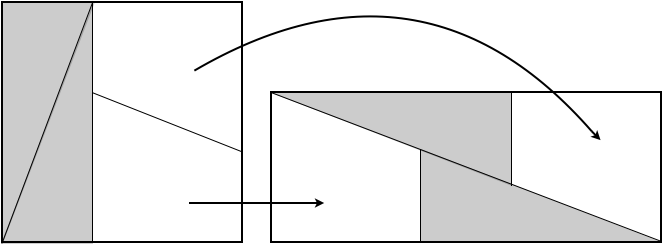
\includegraphics[scale=0.4]{FiguresMaths//FiboParadox.png}
              \caption{Construction of the rectangle after splitting the $8 \times 8$ square
              in two right $8$ by $3$ triangles and two polytopes.}
        \label{fig:FiboParadox}
\end{center}
\end{figure}

The surface of the square is $F(n)^2$ while the rectangle is $F(n+1).F(n-1)$.
In Fig.~\ref{fig:FiboParadox}, the Cassini identity is applied for $n=5$, $F(5)=8$. 
On one side, we obtain a surface of $8 \times 8 = 64$, but $13 \times 5 = 65$ on the other side!
What's wrong?

The paradox comes from the wrong representation of the diagonal of the rectangle which does not coincide with the hypothenuse
of the right triangles of sides $F(n+1)$ and $F(n-1)$.
In other words, it always remains (for any $n$) an empty space (corresponding to the unit size of the basic square of the chess board).
The greater $n$, the better the paradox because the deformation of the surface of this basic square becomes more tiny. 


%\subsection{Using Fibonacci numbers}
%
%$F(n)$ is the number of paths from node $1$ to $n$ in the following family of graphs of figure~\ref{fibograph}. 
%
%\begin{figure}[h]
%\begin{center}
%        \includegraphics[scale=0.4]{../FIGmaths/FiboGraph.pdf}
%        \caption{Counting paths from node $1$ to node $n$ ($n=7$)}
%        \label{fibograph}
%\end{center}
%\end{figure}
%%Show how this number is related to Fibonacci's numbers.
%%\item Find a closed form for the sum of consecutive Fibonacci numbers.




\ignore{***********
\section{The Token Game}
\label{sec:TokenGame}

\subsection{Principle}

%Let us start by studying a puzzle whose solution can be obtained by a recursive algorithm. 

Consider a bank with $n$ circle positions numbered from $1$ to $n$ and $n$ tokens.
Initially, the bank is empty (see Figure~\ref{fig:jeujetonsInit}).
%\begin{itemize}
%\item Put a token in position $1$ if it is empty or remove the token in position $1$.
%\item Put a token in the position 
%\end{itemize}

\begin{figure}[h]
\begin{center}
        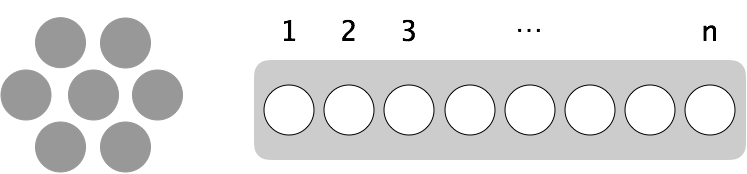
\includegraphics[scale=0.4]{FiguresMaths/GameTokenInit.png}
        \caption{Initial position: $n$ tokens (grey) and all the empty bank.}
        \label{fig:jeujetonsInit}
\end{center}
\end{figure}

The game consists in determining the process to fill the bank with the $n$ tokens, putting or removing one token at a time according to one of the two 
following constraints.
Both rules are illustrated in figures~\ref{fig:rule1} and \ref{fig:rule2}.

\begin{itemize}
\item \textbf{Rule 1.} Position 1: Put a token if it is empty or remove it.
\item \textbf{Rule 2.} Position next to the first empty position (i.e. on the right): Put a token if the position is empty or remove it.
\end{itemize}

Notice that the first rule only refers to positions (and thus, it is symmetric in regard to the move: put or remove a token), 
while the second one is not symmetric.

\begin{figure}[h]
\begin{center}
        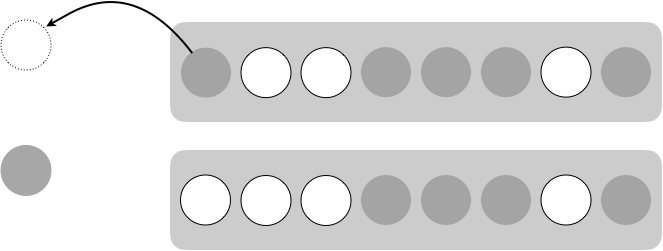
\includegraphics[scale=0.4]{FiguresMaths/GameTokenRule1.png}
        \caption{Rule 1: Position 1 contains a token, thus, remove it.}
        \label{fig:rule1}
\end{center}
\end{figure}

\begin{figure}[h]
\begin{center}
        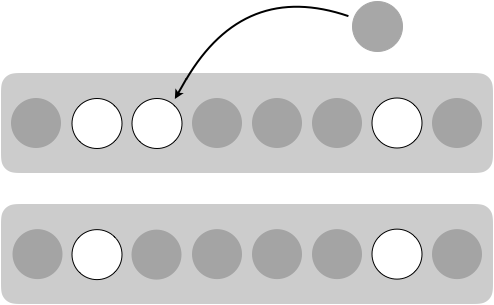
\includegraphics[scale=0.4]{FiguresMaths/GameTokenRule2.png}
        \caption{Rule 2: The position next to the first idle position (i.e. position 3 in this example) 
        is idle, thus, put a remaining token here.}
        \label{fig:rule2}
\end{center}
\end{figure}

The analysis of the game for some particular values of $n$ leads to some evidences (looking at the first ranks):
First, in the even case, the process should start by putting the second token while in the odd case, we should start to fill the first position.
%Then, the first token is flipped every double steps, the second one every four steps and so on.
Second observation: both rules are applied alternatively (this is obvious for Rule 1 since applying it twice consecutively leads to the initial position, 
and easy to check for Rule 2 on the first ranks). 
However, the solution is not easy to describe and its cost is not easy to establish.

The solution can be easily expressed recursively as follows (for $n > 2$):
the token in the last position can only be put bu rule 2, that means that the first $(n-2)$ one are on the bank.
Then, if we empty these first $n-2$ positions,
we obtain a configuration similar as in the initial one except for the last position which has a token. 
Then, the puzzle is solved by applying the same process on a bank with $n-1$ tokens.
The successive steps of this recursive solution are depicted in Figure~\ref{fig:jeujetonsPrinciple}.

%Thus, flipping the first tokens of the same color is different if they are all blue or red.
%Notice that flipping the first reds can be obtained using the reverse process as for the blue ones (see coding at the end of this document).

\begin{figure}[h]
\begin{center}
        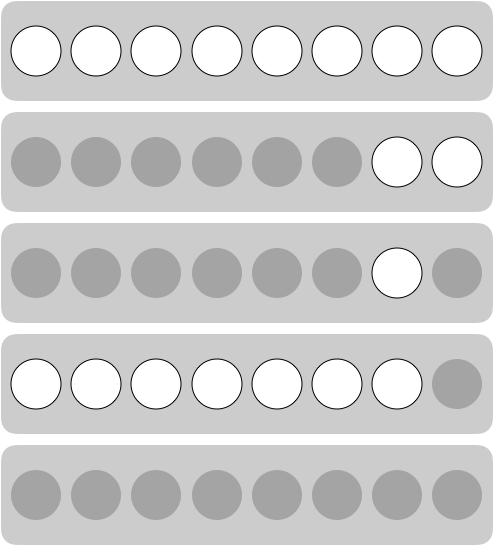
\includegraphics[scale=0.4]{FiguresMaths/GameTokenPrinciple.png}
        \caption{Principle of the recursive solution. Fill the bank in the $(n-2)$ first positions, then, put a token on the last position (Rule 2), 
        empty the (n-2) first positions. Finally, fill the $(n-1)$ first positions of the bank.}
        \label{fig:jeujetonsPrinciple}
\end{center}
\end{figure}
\bigskip

More formally,
\bigskip

fillBank(n)
\begin{itemize}
\item
 if $n=1$ then putToken(1) -- according to Rule 1
\item
if $n=2$ then PutToken(2) -- Rule 2 -- and then PutToken(1) -- Rule 1

\item 
if $n > 2$ then
\begin{itemize}
\item fillBank(n-2)
\item PutToken(n)
\item EmptyBank(n-2)
\item FillBank(n-1)
\end{itemize}
\end{itemize}

\subsection{Analysis}

The analysis comes directly from the previous process. 

Let call $f(i)$ the cost for filling the bank from position $1$ to position $i$
(the cost here refers to the number of elementary moves, put or remove a token).
Notice that it requires the same number of steps to fill or to empty the truncated bank (from position $1$ to $i$). 
The total cost is to fill the whole bank of size $n$, thus we have to solve:

$f(n) = f(n-2) + 1 + f(n-2) + f(n-1) = f(n-1) + 2.f(n-2) +1$ for $n > 2$

with $f(1) = 1$ and $f(2) = 2$.
\bigskip

If we add $f(n-1)$ in both sides of the previous expression, we obtain a simpler equation (call $s(n)$ the sum $f(n)+f(n-1)$ $n \geq 2$,
in particular, $s(2) = 2+1$):

$f(n) + f(n-1) = 2.f(n-1) + 2.f(n-2) +1$

$s(n) = 2.s(n-1)+1 = 2.(2.s(n-2)+1) + 1 = 2^2 s(n-2) + 2+ 1 = 2^3 s(n-3) + 2^2 + 2 + 1 = ... = 2^{n-2} s(2) + 2^{n-3} + ... + 2^2 + 2 + 1$ where $s(2) = 2+1$

$s(n) = 2^{n-1} + 2^{n-2} + 2^{n-3} + ... + 2^2 + 2 + 1$ 

Summing up this geometric series leads to
$s(n) = 2^{n} -1$
\bigskip

Coming back to the $f(n)$, we can rewrite this equation as:

$f(n) = 2^{n} - f(n-1) -1$ where $f(1)=1$

$f(n) = 2^{n} - 2^{n-1} + f(n-2) +1 -1 = 2^{n} - 2^{n-1} + 2^{n-2} - f(n-3) -1 = ...$

This sequence is an alternate series of the powers of $2$ where the $1$ and $-1$ are cancelled two by two.
However, there is a different number of steps if $n$ is even or not. 
In this case, the last term is $-2$, while it is $-1$ when $n$ is odd.
\bigskip

For $n$ even, $f(n) = \sum_{1 \leq k \leq n}(-1)^{k}2^{k} $

For $n$ odd, $f(n) = \sum_{0 \leq k \leq n}(-1)^{k+1}2^{k} $
\bigskip

$f(n)$ is an alternate series of the successive powers of $2$, which can be solved by a graphical proof.

We rewrite it by gathering the positive and negative terms as follows (for odd $n$): 
$f(n) = (2^{n} + 2^{n-2} + ... + 2) - (2^{n-1} + 2^{n-3} + ... + 1)$

$= 2.(2^{n-1} + 2^{n-3}  + ...  +1) - (2^{n-1} + 2^{n-3}  + ... + 1)$

$= 2^{n-1} + 2^{n-3}  + ...  +1$ 

Consider first the odd case (here, $2^{n+1}$ is a perfect square).
Figure~\ref{fig:alternatePowers2odd} gives a representation of $f(n)$ 
where the smallest surface at the right is the unit square.

Take 3 copies of $f(n)$ as it is depicted in figure~\ref{fig:alternatePowers2finalOdd},
two are mirror configurations and the third one (represented in grey) fills the remaining part of a big square but some idle space at the 2 extreme right corners. 
The whole surface is a perfect $2^{n} \times 2^{n}$ square, equal to $2^{n+1}$ plus the small surface equal to half of the basic unit square ($2 \times \frac{1}{2}$ = 1). Thus, $3.f(n)+1= 2^{n+1}$.

\begin{figure} [h]
\begin{center}
        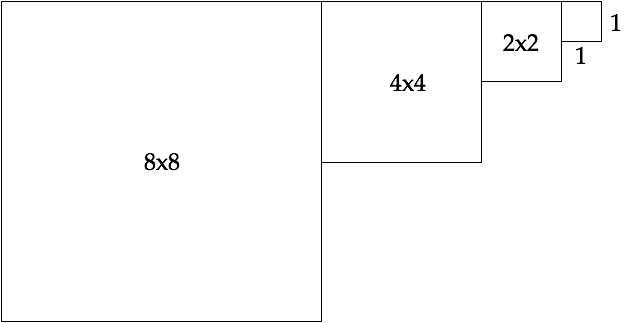
\includegraphics[scale=0.4]{FiguresMaths/alternatePowers2initOdd.png}
        \caption{Representation of the alternate series of powers of $2$ for $n=7$.
        f(7)=64+16+4+1.}
        \label{fig:alternatePowers2odd}
\end{center}
\end{figure}

\begin{figure} [h]
\begin{center}
        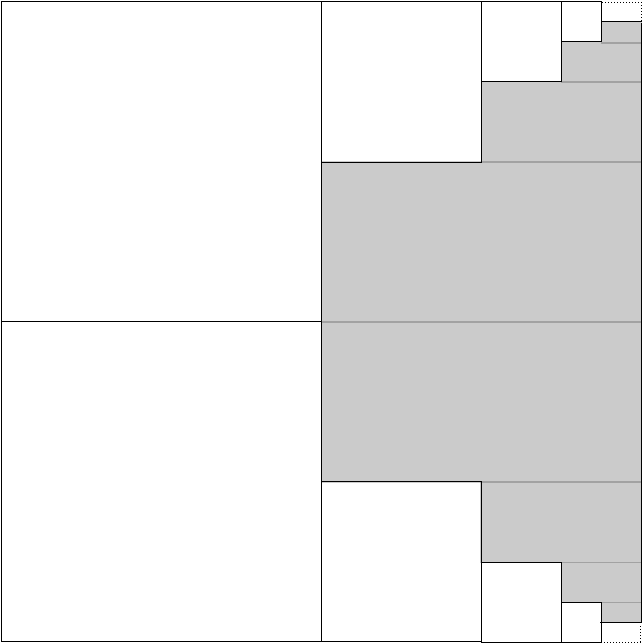
\includegraphics[scale=0.4]{FiguresMaths/alternatePowers2odd.png}
        \caption{Even case: Geometric proof using 3 copies of $f(n)$ that almost fill a large square.}
        \label{fig:alternatePowers2finalOdd}
\end{center}
\end{figure}

The previous construction may be adapted in the even case in a similar way.
The details are left to the readers. 

We propose below another proof obtained by using the results for the odd case:

We start by the expression $f(n) + f(n-1) = 2^n -1$
that is $f(2k) = 2^{2k} - f(2k-1) -1$ for even $n=2k$.

Now, apply the final expression of $f$ to $2k-1$, which is odd: $f(2k-1) = \frac{1}{3} (2^{2k+1}-1)$.

$f(2k) = 2^{2k} - \frac{1}{3} (2^{2k-1+1}-1) -1 = 2^{2k} (1-\frac{1}{3}) + \frac{1}{3} -1= \frac{1}{3} (2^{2k+1} -2)$.
\bigskip

%
%Figures~\ref{fig:alternatePowers2even} and~\ref{fig:alternatePowers2finalEven} illustrate the construction in the even case.
%The details are left to the readers. 
%We obtain $3.f(n)+2= 2^{n+1}$ by a similar analysis.
%However, we can deduce directly the even case from the odd case by remarking that $f(2k)=2.f(2k-1) +1$.
%
%This is obtained by the basic relations $f(n) = 2^{n} - f(n-1) -1$ and $f(2k-1) = \frac{1}{3} (2^{2k} -1)$.
%
%$n=2k$, $f(n) = 2^{2k} - \frac{1}{3} (2^{2k} -1) -1 = \frac{1}{3} (2^{n+1} -2)$.
%
%\begin{figure} [h]
%\begin{center}
%        \includegraphics[scale=0.4]{FIGmaths/alternatePowers2initEven.png}
%        \caption{Representation of the alternate series of powers of $2$ for $n=6$.
%        f(6)=32+8+2.}
%        \label{fig:alternatePowers2even}
%\end{center}
%\end{figure}
%
%
%\begin{figure} [h]
%\begin{center}
%        \includegraphics[scale=0.4]{FIGmaths/alternatePowers2even.png}
%        \caption{Case odd: Geometric proof in the odd case. Notice here that there are 2 small rectangles left at the extreme corners on the right,
%        whose surface is $1$ each.}
%        \label{fig:alternatePowers2finalEven}
%\end{center}
%\end{figure}

We finally obtain: 

$f(n) = \frac{1}{3} (2^{n+1} -1)$ if $n$ is odd.

$f(n) = \frac{1}{3} (2^{n+1} -2)$ if $n$ is even.

******************}
